\section{Structure of the LHCb Detector}
The Large Hadron Collider beauty (LHCb) detector is a single-arm spectrometer possessing a forward angular coverage from
approximately 10 mrad to 300 (250) mrad in the bending (non-bending) plane \cite{https://doi.org/10.48550/arxiv.0910.1740}
The structure of the detector is motivated by the fact that both the $b$ and the $\bar{b}$ hadrons are predominantly produced in the
same forward or backward cone. The components that enable the identification of particles, and aid the deduction of their properties include
the vertex locator system (VELO), the tracking system, comprising of a Trigger Tracker (a silicon microstrip detector, TT) located in front 
of the magnet, three tracking stations behind the magnet made up of silicon microstrips in the inner and outer parts (labelled IT and OT respectively),
two Ring Imaging Cherenkov counters (labelled RICH1 and RICH2 respectively), as well as a calorimeter system, comprising of a Scintillating Pad Detector and Preshower
(SPD/PS) and electromagnetic and hadronic calorimeters (ECAL and HCAL respectively) \cite{https://doi.org/10.48550/arxiv.0910.1740}. The layout of the LHCb spectrometer including the relative positions of the components described above, is illustrated in Figure \ref{LHCbDetector}.\\
\\
Of the abovementioned components, the dipole magnet, VELO, and ECAL play a significant role
in the analysis of the decay described in Section \ref{DecayProcess}. The structure of these sections of the
detector is further elaborated on in the sections that follow.
\begin{figure}[H]
    \centering
    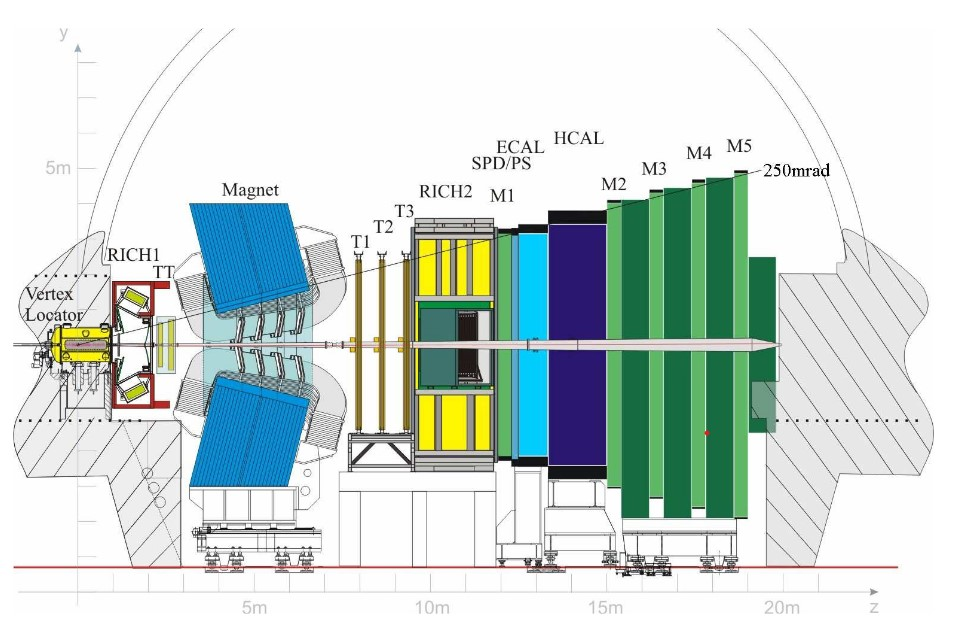
\includegraphics[scale = 0.45]{LHCbDetector.jpg}
    \caption{Diagram of the LHCb detector illustrating its various components. The coordinate system is oriented such that the beam is directed along the $z$ axis, and the $y$ axis is oriented along the vertical. Figure sourced from ADD REFERENCE}
    \label{LHCbDetector}
\end{figure}

\subsection{Vertex Locator (VELO)}
\subsubsection{Angular Coverage}
\subsubsection{Triggering}
\subsubsection{Reconstruction Efficiency}
\subsubsection{Displaced Tracks and Vertices}
\subsubsection{Decay Time}
\subsection{Ring Imaging Cherenkov (RICH) Detector}
\subsection{Magnet} 
\subsection{Electromagnetic Calorimeter (ECAL)}
\section{Data Analysis at the LHCb}
\subsection{The LHCb Data Flow}
\subsection{The LHCb Simulation Framework}
\subsubsection{Gauss}
\subsubsection{EvtGen}
\subsubsection{Pythia}
\subsubsection{Geant4}
\subsubsection{Boole} 



